\documentclass[../intro.tex]{subfiles}
\begin{document}
\section{Notation \& Definitions}
\begin{figure}
    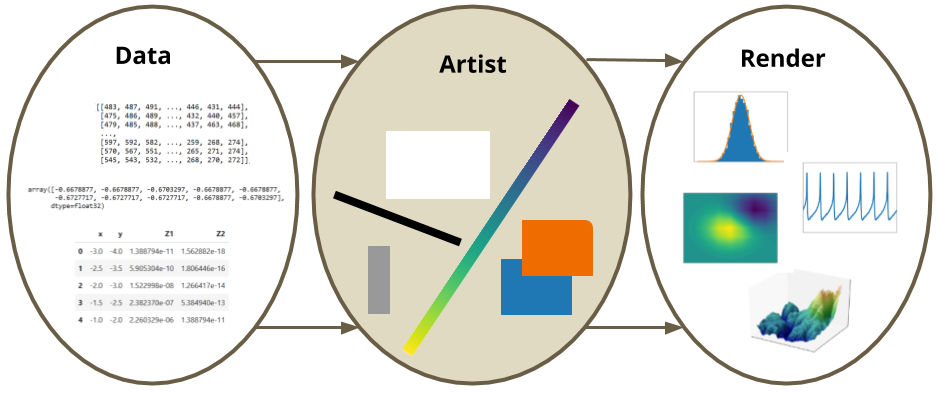
\includegraphics{figures/sections/dar.png}
    \caption{Data with semantic structure (such as tables and images) is mapped to visual encodings (color, position) that are composited into visual idioms (scatter, line) that are rendered into graphics (rasters, vectors).}
    \label{fig:artists}
\end{figure}
Figure~\ref{fig:artists} shows transformation from data into rendered graphical object, wherein there is an intermediate artist stage where the data gets transformed into a visual form. We argue that a faithful representation of the data is one where:
invariance:
functor
* types: variables measurement groups are  with visual encoding groups
* topology: visual idioms preserve the topology/connectivity of the dat


We propose that the mapping of a precise subset of data to a visual idiom ($I$) can be encapsulated in a class of functors called artists.

\begin{equation}
    A: \Gamma(V) \mapsto 
\end{equation}

%% cw versus list of pixels for the connectivity?
    %% toplogical spaces allow you to encode connectvity/continuity 
%% anypoint on the cw complex I can hook into R7 to get back the {color, alpha, position}
%% has functions that take it into R7 (lookup table for the spec (raster, vector))
%% vector represention is the CW 
%% f:T\mapsto \mathbb(R^{7}), T \in CW
%% this function is never called w/ elements in T
%% T is embedded in f, is the topology of the thing on the screen (scene graph?)
%% output of artist has no semantic meaning, is the line representation of the visual idiom 
%% in what sense are we preserving continuity on dotted lines? 
\subsection{data}
We use fiberbundles as our underlying data representation because it concisely encodes topology\cite{butlerVectorBundleClassesForm1992,butlerVisualizationModelBased1989} and type \cite{spivakSIMPLICIALDATABASES}. 
For example, the iris dataset \cite{UCIMachineLearning} has a topology of disconnected points (k=0) and variables of type nominal (species type), and ratio (sepal and petal length and width). To encode this in a formal way, we rely on Butler's 

Types and topology are (statement is line of equation)


\end{document}